\newpage
\section{Dynamic exposure \& health studies}
\label{sec:dynamicexposurehealth}

As we have seen from the studies reviewed thus far, effectively and accurately quantifying human exposure to air pollution for epidemiological studies is fraught with problems. Studies that look at sufficiently large numbers of subjects find it difficult to accurately assign exposure to them, as the subjects spend time in many different environments, travel between these micro-environments, and often the air quality data is of insufficient temporal or spatial quality. The epidemiological studies that are based upon these estimations may therefore be making incorrect health conclusions. \cite{Brauer2002} measured personal exposure compared to monitoring site exposure for PM$_{2.5}$ for 16 subjects in Canada and found that in 13 of the 16 subjects the measured ambient concentrations were under-representing exposure. Ashmore's review of literature focusing on children's exposure found that their exposure is closely related to concentrations in the home, at school, and in transport --- differing significantly from adults concentrations and general outdoor concentrations such as those at monitoring sites (\cite{Ashmore2009}). Although the links between health and air pollution are fairly clear as was discussed in section \ref{sec:healtheffects}, it might be that this miss-classification error is biasing calculated risk factors, regressions or coefficients towards the null value (no association) i.e. once exposure classification is improved the relative risks of increases in exposure to pollutants may be greater than previously thought (\cite{Armstrong1990}).

%%%%%%%%%%%%%%%%%%%%%%%%%%%%%%%%%%%%%%%%
%%%%% PERSONAL MONITORING %%%%%%%%%%%%%%
%%%%%%%%%%%%%%%%%%%%%%%%%%%%%%%%%%%%%%%%

\subsection{Personal Monitoring}
\label{sec:personal_monitoring}

To gain further insight and a more realistic understanding of individual-level exposure to pollutants, personal monitoring methods can be used. Studies that are described as personal monitoring vary in their use of equipment, and measuring of different pollutants, but generally describe studies that attach portable pollutant monitoring devices to a person or persons, who then go about their normal lives while the devices collect data. The devices normally collect data at short time intervals i.e. one minute, and are combined with location devices like a GPS. By using these devices the researchers are able to collect data on concentrations at the the places that the subjects are in, and see how levels vary between them. Using such equipment, individual level objective direct measures of exposure can therefore be collected. These studies are considered the "gold standard" of exposure assessment (\cite{Ashworth2013} , \cite{DeNazelle2008}) .

\cite{Steinle2013} conducted a review of personal exposure studies of this style. They discussed the difference between traditional exposure assessments using fixed air quality network sites, single micro-environments and static populations, compared to the new developments in sensor technology that have enabled researchers to directly monitor pollutants while people move through varying concentration fields and activity space. They summarised the personal exposure approach with Figure \ref{fig:traditional_personal_monitoring} which visualises the joining of location data and concentration data

\begin{figure}[H]
\centering
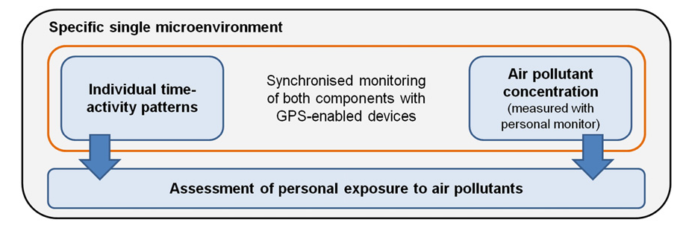
\includegraphics[scale=0.7]{traditional_personal_monitoring}
\caption{Conceptual model illustrating the traditional approach for the assessment of personal exposure to air pollution \cite{Steinle2013}}
\label{fig:traditional_personal_monitoring}
\end{figure}

This area of air pollution exposure research has, as Steinle notes, accelerated in popularity recently due to the advancements in related technology. The devices have become cheaper, lighter and easier to collect/process data from. The ubiquitous nature of smart phones has also contributed in terms of it becoming the norm for people to carry about technology and have elements of their lives tracked. Indeed, studies such as \cite{DeNazelle2013} have used data from smartphone applications that are not designed for exposure assessment, but which offer a rich data set (the application CalFit for estimating peoples movements style i.e. running, cycling, walking). A search of the terms "'personal exposure' AND 'air pollution'" in PubMed, summarised by year of publication in Figure \ref{fig:personal_exposure_publications} nicely illustrates the rise in these studies (whilst acknowledging that there are mitigating circumstances such as the popularity of the field as a whole, and numbers of journals in this area etc.):

\begin{figure}[H]
\centering
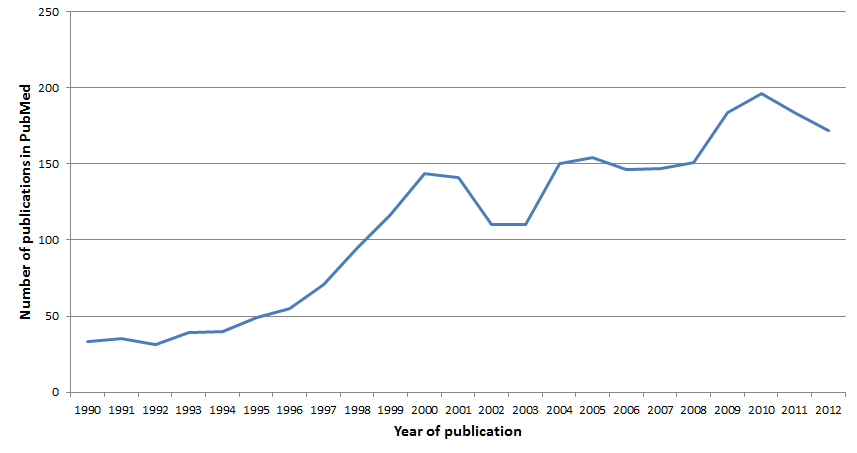
\includegraphics[scale=0.6]{personal_exposure_publications}
\caption{Numbers of publications about personal exposure to air pollution in PubMed}
\label{fig:personal_exposure_publications}
\end{figure}

\cite{Dons2011} in Belgium completed personal monitoring campaigns for 16 couples. One member of each couple was identified as a full-time worker, and one as a homemaker. Each couple's personal exposure was measured over 24 hours by them carrying a micro-aetholometer and a PDA device which contained a GPS chip for location and time-activity diary for contextual information (which was subsequently completed by the individuals). Very different patterns of exposure were observed between the couples, despite them living in the same place i.e. two individuals living in the same location would have the same exposure according to some of the approaches in the static studies section. Exposure differed by upto 30\% between couples, with exposure during transport being identified by Dons et al. as the most important factor in this discrepancy. In a similar study in Italy \cite{Buonanno2014} conducted personal monitoring on 24 non-smoking couples  and measured their exposure to UFPs using a Phillips NanoTracer which included a GPS for tracking. In this study the couples were all male-female, the male being a full-time worker and the female being a homemaker. Given the emphasis that Dons found on transport, it was slightly surprising that this study found women to have higher exposure than men. This is attributed to the emissions from cooking stoves in the home and that the particles stay in the environment for prolonged periods. Although the two studies actually consider different metrics (black carbon compared to ultrafine particles) so the comparison is hard to make directly -- there are not many sources of black carbon in the home, but transport is a major source outside of the home. In a further study \cite{Broich2011} used a GPS, and GRIMM 1.09 monitor to measure particulate matter (in various sizes) for sixteen people over 24 hours each in Italy.

\begin{figure}[H]
\centering
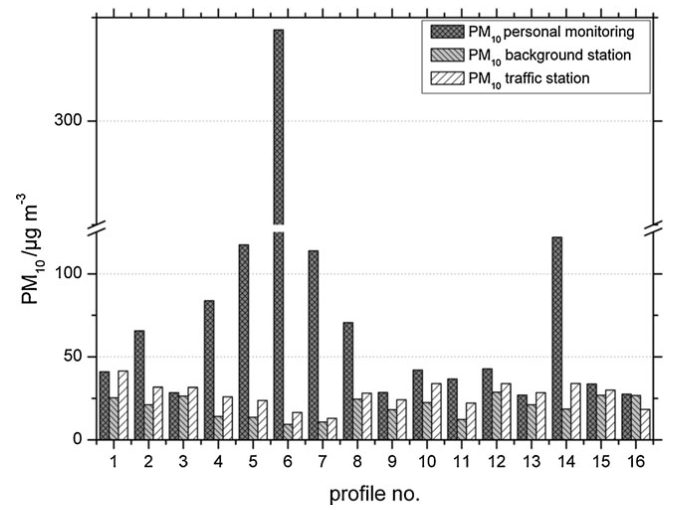
\includegraphics[scale=0.6]{broich_exposures}
\caption{Average exposure over 24 hours to PM$_{10}$, comparing personal monitoring, background monitoring stations and traffic monitoring stations from \cite{Broich2011}}
\label{fig:broich_exposures}
\end{figure}

As can be seen from Figure \ref{fig:broich_exposures}, there were large variations between the personal exposure concentrations and concentrations at nearby fixed-sites. The averages over 24 hour between participants varied from 27 to 322 $\mu \text{g m}^{-3}$, and like Dons they found that exposure levels were heavily dependant on the travel participants undertook, and the micro-environments they spent time in. Broich argues this is why direct personal exposure monitoring is needed for accurate exposure assessments in the future, rather than proxy methods. Although for epidemiological studies that might relate patterns from monitoring sites to patterns in incidents of poor health, this is not necessarily the case. If the personal exposure results for instance are always say 40\% than the monitoring site, then the monitoring sites would still capture the trends and might be able to relate these trends to hospital admissions. 

While these types of study are excellent at providing hyper-local and time resolved personal exposure data, they tend to struggle to provide data that is useful for considering alongside the harmful health effects of poor air quality. The studies give results for individuals or small groups of people which are not able to be used alongside health-related epidemiological data such as hospital admission records or incidences of asthma in a certain region. As \cite{Chaix2013} argues, improving measuring of exposure to environmental conditions by accounting for the movement of individuals is critical, however by using such small numbers I suggest that there is a danger of over-generalisation between exposure and health. Measuring 20 school-children's exposure to PM$_{10}$ for example, and then making wide-ranging assumptions about the health effects of PM$_{10}$ on school children seems simplistic. It might be that those 20 children are in the top 5\% of exposures and not a good representation of school children in general.

\cite{Steinle2013} argues that the trend in the area of calculating accurate exposure estimates for large populations is for the development of the personal monitoring approach, i.e. distribution of low-cost, accurate GPS devices combined with accurate low-cost unobtrusive portable air quality measurement devices. In this way the amount of data collected through this 'gold-standard' method would be adequate to allow extrapolation to large groups of people. A model of their theoretical approach is shown in \ref{fig:steinle_full_assessment}.

\begin{figure}[H]
\centering
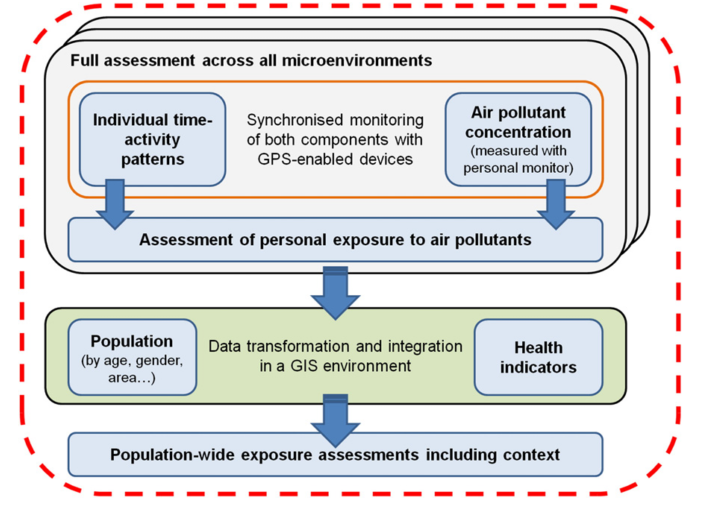
\includegraphics[scale=0.8]{steinle_full_assessment}
\caption{Conceptual model for the assessment of individual and population-wide exposure to air pollution including effects from \cite{Steinle2013}}
\label{fig:steinle_full_assessment}
\end{figure}

\cite{Minguillon2012} agree with them after their study on pregnant women's exposure in Barcelona in 2009. They compared measurements from the subjects household balcony, inside their house, and the data from personal monitoring equipment. They found mean concentrations for PM$_{2.5}$ of 20 ug/m\textsuperscript{3}, 24 ug/m\textsuperscript{3}, and 27 ug/m\textsuperscript{3}, for outdoor, indoor, and personal samples respectively. They concluded that it was important to rely on personal exposure measurements for epidemiological studies.

However I would argue that this is not currently practical. The technology for this type of study is not yet available, as the authors themselves note. In addition, even if it were, the distribution of the devices and automated collection of the data on a large enough scale seems difficult to achieve. Though this may change with the advent of smaller and lower-cost measurement technology.

What the personal monitoring studies in this section do show the researchers in this field is where subjects spend alot of their time (indoors), and where they are exposed to the highest levels of air pollutants (travel). They emphasise how important these factors are in understanding the true exposure of individuals compared to current or traditional methods. Developing a modelling approach, with focus on the accuracy of the model in these places, to improve exposure estimates, seems to be a more attainable goal. Understanding exposure in these micro-environments for input to such models is therefore crucial.

%%%%%%%%%%%%%%%%%%%%%%%%%%%%%%%%%%%%%%%%
%%%%%%%%%% INFILTRATION %%%%%%%%%%%%%%%%
%%%%%%%%%%%%%%%%%%%%%%%%%%%%%%%%%%%%%%%%

\subsection{Infiltration}
\label{sec:infiltration}

%% What is infiltration
Infiltration refers to the diffusion of outdoor air into the environment inside a building. The amount of outdoor air that moves inside depends on ventilation, air conditioning and on the indoor--–outdoor temperature gradient. EU guidelines now state that buildings must be insulated to save energy, however as buildings allow less air to be exchanged with the outside environment, the indoor concentration of pollutants can increase if there are significant indoor sources. Thus increasing the air-tightness of buildings can have negative impacts on health (\cite{Gens2014}). This is offset of course by meaning that harmful outdoor pollutants will also not as easily infiltrate into the indoor environment. The study of indoor air has become an inherent part of modern exposure research (\cite{Steinle2013}). Figure \ref{fig:infiltration} below illustrates how outdoor air infiltrates buildings and mixes with indoor air.

\begin{figure}[H]
\centering
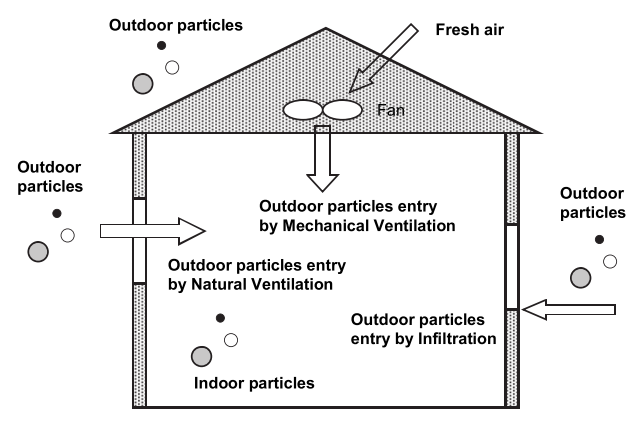
\includegraphics[scale=0.7]{infiltration}
\caption{Infiltration from \cite{Chen2011}}
\label{fig:infiltration}
\end{figure}

Indoor pollutants have many sources such as cigarette smoke, cooking, heating and cleaning products. They can substantially modify a persons exposure and characterisation of them is difficult and complex. To consider the exposure of subjects to air pollution over days/weeks/months, indoor air is an important consideration.  A better understanding of the factors influencing infiltration and indoor sources will improve exposure assessment methods and contribute to reduced exposure miss-classification in epidemiological studies (\cite{Colbeck2010a}, \cite{MacNeill2012}). Although this of course depends on the metrics that are being used for considering the health effects -- to better understand the effects of traffic pollution on health for example indoor sources would not be needed and the infiltration to the indoor environment would be key. But for a model which considered exposure to all pollutants then all sources would be needed.

%% Some studies that have looked at indoor concentrations
To try and better understand the differences between indoor and outdoor pollution, as part of a large cohort exposure study in Ontario (Canada), \cite{MacNeill2012} measured concentrations of PM$_{2.5}$, UFPs, black carbon and humidity both inside properties and in the back garden of properties at the same time for a period of two weeks.

As is common with this type of study the results were discussed in terms of indoor\slash outdoor ratios, otherwise known as I\slash O ratios. This is the concentrations inside the property, divided by the concentrations outside of the property. So if a property had a PM$_{2.5}$ I\slash O ratio of 0.5 at 10am and the concentrations outside were 10 ug\slash m\textsuperscript{3}, then this would mean that concentrations inside the property were 5 ug\slash m\textsuperscript{3} (10 multiplied by 0.5).

The median daily estimates found in the study ranged from 0.26 to 0.36 across seasons for PM$_{2.5}$, with the ranges typically related to window-opening behaviours, air conditioning, meteorological variables, home age, use of electrostatic precipitators and stand alone air cleaners. The determinants of indoor source concentrations were related to cooking, candle use, supplemental heating, cleaning, and number of people in the home. Expanding on the last of the variables noted by MacNeill, \cite{Colbeck2010a} comments on the close relationship between indoor concentrations and human activities, stating that humans are responsible for their own "personal cloud", that is, exposure to airborne particles resulting from their activities (e.g. occupation, hobbies) or physical activities (e.g. jogging, vacuum cleaning).

\cite{Challoner2014} looked at PM$_{2.5}$ and NO$_{2}$ concentrations in ten different city centre buildings in Dublin. They found PM$_{2.5}$ I/O ratios close to 1 (similar to outside) for the ten commercial buildings, however after studying the temporal variation in these levels they suggested that, in general, indoor sources and/or re-suspension of PM$_{2.5}$ seemed to have a more significant impact compared to variations in outside air quality. \cite{Kearney2014} measured PM continuously for seven consecutive days in 74 Edmonton (Canada) homes in 2010. Simultaneous measurements of outdoor (near-home) and ambient (at a central site) concentrations were also measured. As with the studies above, they found considerable variability ranging from 0.10 to 0.92 in winter and from 0.31 to 0.99 in summer.

Given the number of variables that seem to contribute to variation in indoor air quality, making broad-sweeping assumptions to create inputs to epidemiological models seems difficult. However WHO calculated in 2005 that people spend 89\% of their time indoors, \cite{Lai2004a} found a figure of (89.5\%) from their research, and \cite{Schweizer2007} found similar - 20.66 hours (86\%). Efforts to better quantify this exposure relationship and create as accurate a picture of exposure are therefore needed. The variability in I/O ratios within and between homes may cause substantial exposure miss-classification compared to only using ambient measurements (\cite{Kearney2014}).

So a dynamic exposure model, one that is going to take account of different micro-environments where people spend their time, needs to attempt to model concentrations indoors (given putting time resolved monitors in every indoors environment is impractical). The following paragraphs therefore consider a few recent studies that have attempted to do that.

MESA-Air stands for the "Multi-Ethnic Study of Atherosclerosis and Air Pollution" and is a large research project based in Washington State (USA). The project is designed to examine the relationship between air pollution exposures and the progression of cardiovascular disease (\cite{Allen2012}). To do this they needed to be able to quantify exposure to indoor air, and so they aimed to develop models to predict I/O ratios for around 6,000 homes. They did this by collecting 526 two-week, paired indoor–-outdoor PM$_{2.5}$ filter samples from a subset of homes in their study. Taking account of specific weather and seasonal variables, as well as using information from questionnaires, they made a regression model which predicts I/O ratios (mean of 0.62, SD of  0.21) using easily obtained variables. This is an important study in the cross--over area of air pollution exposure assessment, indoor--outdoor concentrations and epidemiology as it was the first study with a large number of subjects to incorporate variation in residential exposure into exposure assessment. The effect that this new information made to epidemiological study of the prospective cohort is not yet published.

\cite{Hussein2014} took a similar approach with their exposure model, however they also consider dose (Figure \ref{fig:husseiniomodel}). This model calculates exposure by considering infiltration into the indoor environment, indoor sources, building types, building sizes and the time-activity pattern of the individual. A mass-balance model is used for the indoor exposure which not only models infiltration but the indoor sources.

\begin{figure}[H]
\centering
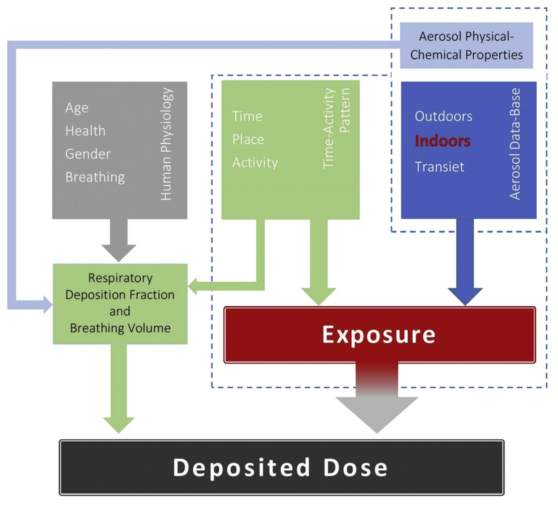
\includegraphics[scale=0.7]{hussein_io_model}
\caption{Exposure model incorporating indoor exposure by \cite{Hussein2014}}
\label{fig:husseiniomodel}
\end{figure}

They illustrate the use of their model by calculating exposure and dose for 24 hours for a test individual, showing the inputs needed for the various model parameters. The advantage of this approach is that it starts to show a way for indoor exposure to be properly included in an exposure assessment model, however as the authors acknowledge the detail and amount of data required for input to the model (i.e. volumes of buildings, detail of indoor sources, time activity patterns) is not yet available on a large enough scale and robust enough, to expand this approach to large numbers of subjects. Lacking exposure modelling of the journeys between the environments would also seem to be necessary for this model to give a more holistic picture of exposure. However the inclusion of the calculation of dose in such a dynamic exposure model is clearly a positive step. Dose being a quantification of the amount of pollutant(s) that the subject actually breathes in and makes its way to the airways and lungs of the subject as per the discussion and diagram of \cite{Brook2010} in Section \ref{subsec:anoverview}.

\cite{Johnson2012} also developed a dynamic exposure model that considered pollutant levels in indoor micro-environments, specifically focusing on NO$_{2}$. They had 60 school-children (ages 12--13) wear personal monitors for two days and while doing so keep a detailed log of their activity, location, and the activity of others around them that might generate pollutants e.g. their parents cooking or smoking at home. Using the time-activity patterns, modelled outdoor concentrations and I/O ratios from literature (e.g. 2 for cars/buses, 0.5 for school) they calculated exposure for the set of children and compared it to their monitored data. The results of this "microenvironmental exposure model" (MEEM) agreed well with the personal exposure measured by the children, however a great deal of contextual information was required to come to such close agreement and it is hard to see how model the could be applied to a much larger cohort of subjects without the same level of detail. Given this the transferability of the study to other subjects and areas is not useful as a tool in and of itself, but it does show that good agreement can be obtained between modelling and monitoring of PE given sufficient data. An additional problem with using this approach elsewhere is that the air quality data was based on a LUR model, which as was discussed in Section \ref{subsec:landuseregression}, requires extensive monitoring to be accurate and often lacks temporal variation (though this study sought to overcome that issue with diurnal profiles from a local monitoring station).

As discussed earlier in this research, the health effects of exposure to air pollution are not yet fully understood. Studies have tended to assign exposure based on outdoor concentrations at the subjects residence using long term average concentrations or on monitoring stations concentrations for studies of short-term exposure. Given this it is no surprise that the negative effects of poor indoor air quality on a populations health are similarly not yet understood (although the approaches discussed in the preceding paragraphs are contributing to a better of understanding of overall exposure i.e. they are starting to contribute to understanding and quantifying exposure indoors, while other studies that quantify exposure in other environments are completing the picture).

\cite{Gens2014} is one of very few studies that have attempted to consider how indoor air is affecting health, specifically looking at the increase in air-tightness of modern EU buildings. The assessment was based on modelling exposure to fine particles originating from both outdoor and indoor air, including environmental tobacco smoke. Exposure response relationships were derived and the results showed an increase of adverse health effects in all considered countries (ranging for health effects from 0.4\% in Czech Republic to 11.8\% in Greece for 100\% insulated buildings) due to an accumulation of particles indoors. Unsurprisingly considering only the effects of outdoor air led to a decrease of adverse health effects.  Although the conclusions drawn for this response relationship seem in doubt as the odds-ratios have been applied to the combination of indoor and outdoor air, when they are only designed and suitable to be used for outdoor air.

\cite{Chen2011} conducted a review of modelling approaches on the relationship between indoor and outdoor particles and summarised that I/O ratios vary considerably due to the difference in size-dependent indoor particle emission rates, the geometry of the cracks in building envelopes, and the air exchange rates. Concluding that due to this it is difficult to draw uniform conclusions on I/O ratios, as they vary so much between building types.

The studies discussed in this section show that indoor air varies considerably from outdoor air, and that research is ongoing as to how to effectively model this as one part of a holistic exposure model that also incorporates other environments such as different transport modes. Research so far has identified that indoor air quality is effected by outdoor concentrations, the number and activity of people inside the building (particularly apparent for particulates), the ventilation systems (or lack of), indoor sources, meteorology and the air-tightness of the building.

%%%%%%%%%%%%%%%%%%%%%%%%%%%%%%%%%%%%%%%%
%%%%%%%%%%%%% TRANSPORT %%%%%%%%%%%%%%%%
%%%%%%%%%%%%%%%%%%%%%%%%%%%%%%%%%%%%%%%%

\subsection{Transport}
\label{sec:transport}

As briefly discussed in Section \ref{subsubsec:invehicle}, air quality when in transport can differ greatly from general ambient concentrations. Table \ref{tab:adams_transport_means} in the same section showed measurements in different transport modes by \cite{Adams2001}, which were different (mostly higher) than that of the ambient concentrations at the time. The recent review of pollutant concentrations in different transport modes by \cite{Karanasiou2014} provides an excellent resource for considering the breadth of the differences between transport and ambient concentrations. Reflecting transport exposure as part of a persons total exposure is important as it is thought that individuals gain a significant contribution of their daily exposure from it, despite the small percentage of time of the day that is spent doing it. For black carbon exposure \cite{Dons2011} found subjects spent 6-8\% of  their day in transport, where they accumulated 21\% of their exposure, and approximately 30\% of inhaled dose. Failing to account for these important exposure events will lead (does lead) to miss-classification in epidemiological studies. 

As can be seen from the data compiled by the Office for National Statistics in figure \ref{fig:transportprofiles}, the three most popular modes of transport in England and Wales over the last half a century have been car and van, followed by bus and coach, and finally rail. 

\begin{figure}[H]
\centering
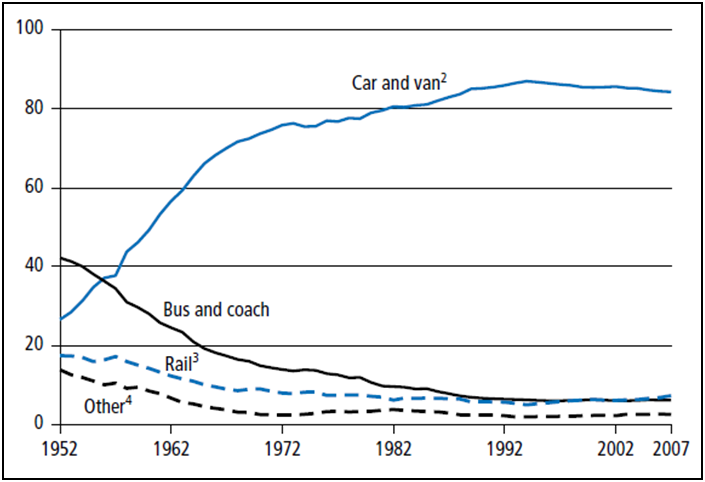
\includegraphics[scale=1]{transport_profiles}
\caption{Transport profiling from ONS census data}
\label{fig:transportprofiles}
\end{figure}

Studies which have sought to measure and understand exposure in these transport modes are now discussed, with the addition of cycling. Cyclists are included as a special case due to their increased inhalation rates and proximity to road traffic which may significantly increases their exposure and dose of poor air quality.

%% A paper here that I've been given after this was done that might want to include. It's about exposure in transport.
%% http://www.arb.ca.gov/research/seminars/zhu/zhu.pdf

%%%%%%%%%%%%%%%%%%%%%%%%%%%%%%%%%%%%%%%%
%%%%%%%%%%% BUS AND COACH %%%%%%%%%%%%%%
%%%%%%%%%%%%%%%%%%%%%%%%%%%%%%%%%%%%%%%%

\subsubsection{Bus and Coach travel}
\label{sec:bus_and_coach}

The review by \cite{Karanasiou2014} found that pollutant concentrations inside bus and coach vehicles vary greatly by country, reflecting the variation in weather conditions, vehicle types, ambient concentrations, and fuel sources of the surrounding fleet. In one study concentrations in the Netherlands were found to be higher in diesel vehicles than on the same routes with electric fuelled buses, suggesting that the own vehicles exhaust impacts on the exposure inside the vehicle. Though this could also be reflective of the permeability of the vehicle or the number of times the doors were opened or closed. In comparison to ambient concentrations, a Paris study found an I/O ratio of 1.3, and in the Netherlands a similar ratio of 1.43 . Typical PM$_{2.5}$ concentrations inside the vehicle across the eleven studies reviewed were in the range 35 -- 69 ug/m\textsuperscript{3}.

A study not covered in the review is by \cite{Song2009} in York, U.K. Measurements were made simultaneously by placing an optical particle monitor in the middle of a bus in York over a period of three days in May 2007, and comparing the data recorded to measurements from an identical monitor on the bonnet of a car which followed the bus (\cite{Song2009}). Measurements were completed during the morning and evening rush hours over 24 hours. Figure \ref{fig:bus_ratios} shows how the relationship between out-bus and in-bus concentrations was positively linear, with a higher gradient as particle size increases (the column labelled 'Dependent variable' is the size fraction of PM). Also having the windows closed on the bus actually led to increased concentrations compared with having the windows open, suggested to be due to re-suspension by passenger activity. 

\begin{figure}[H]
\centering
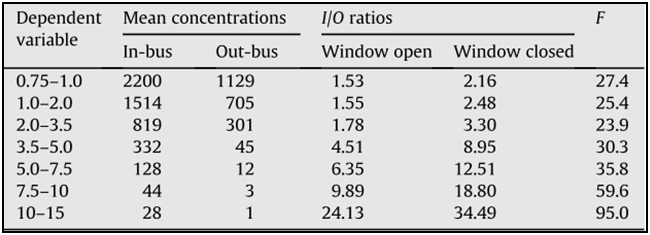
\includegraphics[scale=1.2]{bus_ratios}
\caption{Comparison of mean in-bus and out-bus particle concentrations}
\label{fig:bus_ratios}
\end{figure}

I/O ratios for PM in the size range of 0.75 to 2.0 are 1.53 and 1.55 for when the windows are open, and 2.16 and 2.48 for when the windows are closed. There are many other factors which complicate drawing conclusions between studies, but it is interesting to note how closely the former of these ratios agree with the studies in Paris and the Netherlands for similar PM fractions discussed at the start of this section. 

Using data from this study, the \cite{Song2009} paper concludes by compiling a model for estimating the indoor/outdoor ratio of different PM fractions. The model showed broad agreement with measured particle concentrations inside buses and demonstrated that re-suspension by passenger activities and deposition to the surface of the passengers had significant effects on the concentrations.

The health implications of bus and coach exposure is not discussed by the Karanasiou review or the Song paper as a separate issue or metric. Being able to include exposure by this transport mode in a large-scale exposure assessment exercise is required for exposure mis-classification to be reduced. Though is further complicated, as in many of the sections of this report, by the composition of particles i.e. particles from different sources have more or less harmful effects on health.

%%%%%%%%%%%%%%%%%%%%%%%%%%%%%%%%%%%%%%%%
%%%%%%%%%%%%% CAR TRAVEL %%%%%%%%%%%%%%%
%%%%%%%%%%%%%%%%%%%%%%%%%%%%%%%%%%%%%%%%

\subsubsection{Car travel}
\label{sec:car}

Studies on exposure to subjects while travelling inside cars are more frequent than those of other transport modes. From reviewing studies of car exposure \cite{Karanasiou2014} found that typical European PM concentrations inside passenger cars were in the range of 36–-76 ug/m\textsuperscript{3} for PM$_{10}$ and 22-–85 ug/m\textsuperscript{3} for PM$_{2.5}$. Whether the car itself was powered by diesel or gasoline was found in most studies to make little difference to PM, PNC and BC. However \cite{Jalava2012} found that pollutant concentrations inside the car depended highly on the type of fuel used.

A separate review by \cite{Nasir2009} found that exposure to particulate matter in the car micro-environment is largely dependent on traffic congestion, road network layout, vehicle design/condition and ambient concentrations.

\cite{Dons2013} studied slightly different parameters, or ways of considering the parameters, of BC exposure in vehicles in Figure \ref{fig:road_type_exposure}. It was noted that in urban areas concentrations inside vehicles are higher compared to exposure in more rural areas; with the same holding true for highways versus local roads for motorists -- suggesting that the surrounding fleet and traffic speeds affect in-vehicle concentrations.

\begin{figure}[H]
\centering
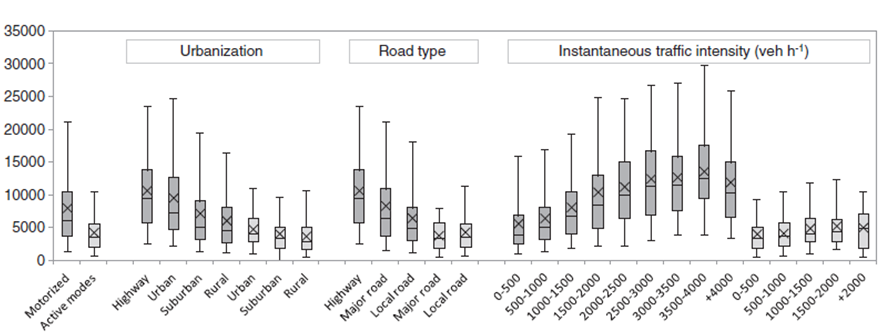
\includegraphics[scale=1]{road_type_exposure}
\caption{External factors affecting in-car BC exposure (ng/m\textsuperscript{3}) from \cite{Dons2013}. Vehicles are the dark boxplots. Walking are light}
\label{fig:road_type_exposure}
\end{figure}

By taking all the factors studied by Dons, a regression model of car I/O ratios for black carbon was developed and is shown in Figure \ref{fig:transport_io_ratios}.

\begin{figure}[H]
\centering
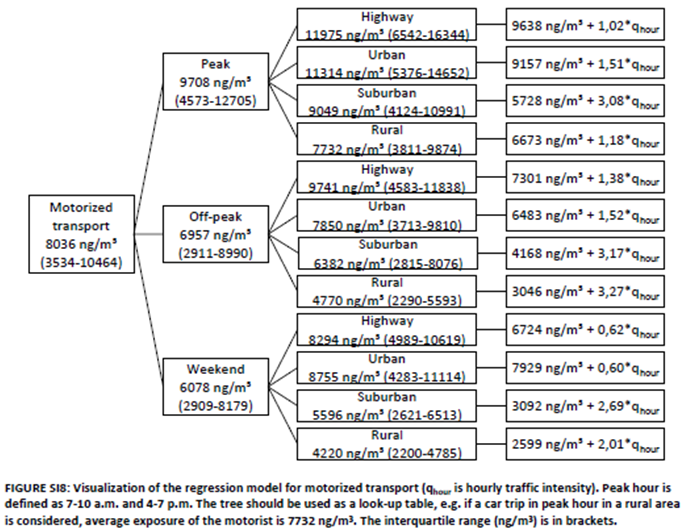
\includegraphics[scale=0.9]{transport_io_ratios}
\caption{Transport indoor/outdoor ratios from \cite{Dons2013}}
\label{fig:transport_io_ratios}
\end{figure}

However the use of these ratios are not well tested and do not always agree with other ratios from the literature. It seems that given other known influences such as ventilation systems that a deterministic model based only on time of day and road type is too simplistic. For example in the two studies by Gulliver and Briggs (\cite{Gulliver2004} and \cite{Gulliver2007}) PM concentrations inside the cars in Northampton and Leicester respectively were roughly 30\% higher than concentrations at nearby monitoring stations (comparisons with immediately outside the vehicles were not available). A table of mean concentrations from the 2004 paper are shown below in Table \ref{tab:gulliver_vehicle_means2}) for reference.

\begin{table}[H]
\centering
    \begin{tabular}{ | l | l |}
    \hline 
     \bfseries{PM Fraction} & \bfseries{Mean (ug/m\textsuperscript{-3})} \\ \hline
     PM$_{10}$ & 43.16\\ \hline
     PM$_{2.5}$ & 15.54\\ \hline
    \end{tabular}
\caption{In-vehicle PM from \cite{Gulliver2004}}
\label{tab:gulliver_vehicle_means2}
\end{table}

The main conclusions from studies on in-car expose were that exposure is significantly influenced by traffic intensity and ambient air pollutant concentrations (being strongly linked to each other) as well as the choice of ventilation used inside the vehicles themselves. Is is a complicated picture. Estimating the exposure of individuals from the time they spend in the car micro-environment should take into account the factors outlined to try and as accurately as possible reflect reality.

%%%%%%%%%%%%%%%%%%%%%%%%%%%%%%%%%%%%%%%%
%%%%%%%%%%%%%%% CYCLING %%%%%%%%%%%%%%%%
%%%%%%%%%%%%%%%%%%%%%%%%%%%%%%%%%%%%%%%%

\subsubsection{Bicycle}
\label{sec:bicycle}

Between 2001 and 2011 the number of people living in London that cycled to work more than doubled from 77,000 in 2001 to 155,000 in 2011. There were also increases in other large UK cities, for example Brighton (increasing by 109\% between 2001 and 2011), Bristol (94\%), Manchester (83\%), Newcastle (81\%) and Sheffield (80\%) (\cite{OfficeforNationalStatistics2014}).

This rise in cycling is due to a number of factors including local authorities building more cycle-friendly infrastructures, the promotion of cycling as a way to keep fit (supported by the Governments cycle-to-work discount scheme), and the public being more environmentally-aware. 

In some cities bicycle sharing systems have also contributed to this rise in cycling journeys. In London the Barclays Cycle Hire scheme was launched in July 2010 with around 5,000 bikes distributed around London at specially installed docking stations (\cite{TransportforLondon2014}). Users were (and still are) able to hire the cycles using a pre-purchased membership key, or by inserting their bank card. Similar systems operate in many places around the World. Although there is no definitive list as new schemes are opening all the time, in 2013 \cite{larsen2013bike} estimated there were more than 500 cities in 49 countries hosting advanced bike-sharing programs, with a combined fleet of over 500,000 bicycles (compared to 213 schemes in 2008 (\cite{Wikipedia2014})).

The \cite{Karanasiou2014} review looked at cycling exposure in 20 European studies, mostly in the UK, the Netherlands and Holland. They found mean exposure values for PM$_{2.5}$ of 29--72 ug/m\textsuperscript{3} and for PM$_{10}$ of 37-62 ug/m\textsuperscript{3}. The London studies (\cite{Kaur2005} and \cite{Adams2001}) found that cycling exposure to PM$_{2.5}$ depended on the route taken, finding busier routes with more traffic increased cyclist's exposure. \cite{Ragettli2013} found similar - bicycle travel along main streets between home and work place contributed 21\% and 5\% to total daily UFP exposure in winter and summer, respectively, and that exposure could be reduced by half if main roads were avoided. At odds with this, the Netherlands study (\cite{Zuurbier2010}) found no difference between routes. Though upon reading their methods in more detail it seems that there was overlap between the low-traffic and high-traffic routes, and also that their low-traffic routes were only low on car traffic and they were frequently used by mopeds.

The main variable affecting cycling exposure was found to be location i.e. a cyclist riding in the middle of a busy road will be exposed to higher concentrations than on a separate cycle-lane. Given cyclists are not enclosed in any sort of vehicle this direct relationship between air pollutant concentration and exposure is to be expected.

With regard to the negative health impacts of exposure to poor air quality while cycling, unlike other transport modes such as car and bus, a number of recent studies have tried to quantify this. \cite{Woodcock2014} used Barclays Cycle Hire data from TfL to model the health impact for 578,607 people in London, mostly (78\%) aged between 14 and 45. They used the bike hire usage data, modelled the journeys between the docking stations, and combined this with general travel data, data on physical activity levels and road collisions, and finally 20 m by 20 m grids of annual average PM$_{2.5}$ data. Cycling exposure was compared to replacing those journeys with walking or public transport. They found that the population benefits from the cycle hire scheme substantially outweighed the negatives, with a net change of minus 72 DALYs among men and minus 15 for women. London’s bicycle sharing system has positive health impacts overall, but these benefits are clearer for men than for women and for older users than for younger users. In a very similar study in Barcelona \cite{Rojas-Rueda2013} did a Health Impact Assessment (HIA) for eight different scenarios where the the population of the Metropolitan area of Barcelona (3.2 million) was presumed to change transport mode from car to either cycling or public transport. Traffic incidents, physical activity and air pollution exposure were then estimated for each scenario and the relative health changes estimated in DALYs. For the scenarios where 20\% and 40\% of car trips where replaced by cycling trips, there were changes of minus 138 and minus 275 DALYs. Rather than doing a health impact assessment \cite{Nwokoro2012}, back in London, did more direct assessments of cycling exposure by looking at the amount of black material in the airways of non-cyclists and cyclists. They found that commuting to work by bicycle in London was associated with increased long-term inhaled dosage of black carbon, however the relationship is difficult to properly quantify. This was because cycling typically takes longer for those people to cycle to work than, for example, a train journey. Route choice further complicates matters as although being away from highly polluted routes would lower exposure, the increased journey time may increase total exposure over the trip. Figure \ref{fig:airway_cycling_blackcarbon} shows the increased macrophage carbon measured in cyclists compared to non-cyclists.

\begin{figure}[H]
\centering
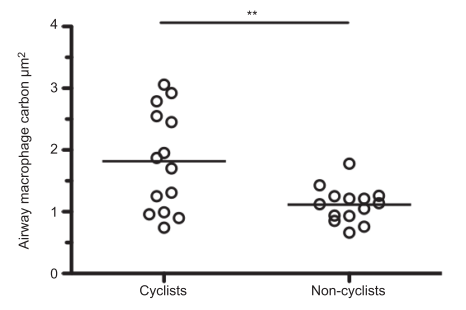
\includegraphics[scale=0.6]{airway_cycling_blackcarbon}
\caption{Airway macrophage carbon in cyclists and non-cyclists from \cite{Nwokoro2012}}
\label{fig:airway_cycling_blackcarbon}
\end{figure}

In summary cycling exposure is very dependant on the routes taken by cyclists, and their position on the road. The negative health effects of cycling have been explored in comparative transport mode studies showing that when taken alongside other variables such as risk of injury, there are overall health benefits to cycling. However there is a lack of studies that take cycling exposure as part of a larger daily exposure health assessment alongside other transport modes and indoor micro-environments. A number of the health studies are encouraging in that they do model sufficiently large groups of people to draw epidemiological conclusions (578,607 people in London and 1.3m in Barcelona) but only the transport aspect of these people's exposure is explored. Also there are other parts of their models which could be improved, for example both studies only used annual average air quality concentrations, and the journeys were not temporally resolved.

%%%%%%%%%%%%%%%%%%%%%%%%%%%%%%%%%%%%%%%%
%%%%%%%%%%%%%%%% TRAINS %%%%%%%%%%%%%%%%
%%%%%%%%%%%%%%%%%%%%%%%%%%%%%%%%%%%%%%%%

\subsubsection{Train travel}
\label{sec:train}

In their 2014 review of commuter exposure in Europe (which has been referred to extensively in this section on transport exposure), Karanasiou did not review train travel -- focusing on cycling, cars and underground subway systems. However \cite{Nasir2009}, \cite{Colbeck2010a}, \cite{Dons2011}, \cite{Ragettli2013} and \cite{Knibbs2011} all have elements of their publications which take train travel exposure as a separate travel microenvironment.

\cite{Nasir2009} and \cite{Colbeck2010a} found concentrations during peak journey times in air-conditioned carriages were 44 ug/m\textsuperscript{3}, 14 ug/m\textsuperscript{3} and 12 ug/m\textsuperscript{3} for PM$_{10}$, PM$_{2.5}$ and PM$_{1}$ respectively, but that during off-peak times, concentrations were about half this. Concentrations were lower again in non-air conditioned carriages. They draw the conclusions that particulate levels inside trains are strongly influenced by the numbers of passengers and that their movement and presence causes particle re-suspension in the air. Peak travel times (when there are more passengers) coincide with high particulate concentrations. Figure \ref{fig:nasirtrainstops} shows the effect of train stops on concentrations in the train cabin. It would have been interesting to see simultaneous outdoor concentrations to see how they varied to the indoor concentrations and more detailed information on passenger numbers. Theoretically it might be that outdoor concentrations contribute to a certain percentage of the indoor concentrations, which are then varied positively or negatively by passenger numbers.

\begin{figure}[H]
\centering
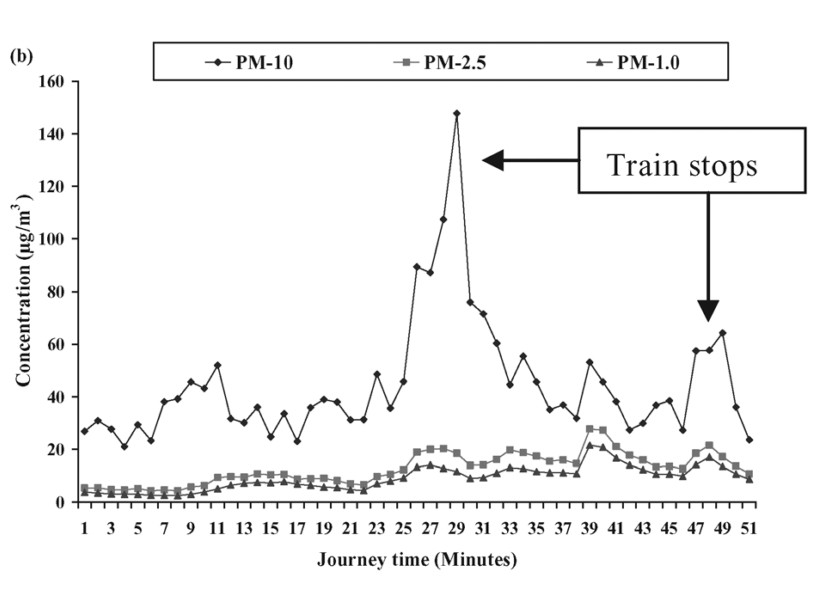
\includegraphics[scale=0.4]{nasir_train_stops.png}
\caption{Train stops and train exposure from \cite{Nasir2009}}
\label{fig:nasirtrainstops}
\end{figure}

\cite{Knibbs2011} reviewed articles to look at the difference between diesel and electric powered trains, and based on the limited data available found that the power source of the rail vehicle appears to strongly affect ultra-fine particle concentrations (diesel powered trains have higher in-train particle concentrations than electric trains). High concentrations of particles are not just confined to the trains themselves either, \cite{Ragettli2013} found ultrafine particle levels within train stations twice as high as suburban background and nearby residential streets in Basel, Switzerland.

In summary the variables that drive exposure levels on trains are the fuel source, the number of stops that the train makes, the influx of passengers at those stops, and the concentrations outside of trains. No research on specifically how train travel exposure affects the health of passengers was found. As with the other transport modes reviewed thus far, a model which incorporates these variables alongside other micro-environments should be able to develop a more accurate picture of human exposure over days or weeks.


%%%%%%%%%%%%%%%%%%%%%%%%%%%%%%%%%%%%%%%%
%%%%%%%%%%%%% UNDERGROUND %%%%%%%%%%%%%%
%%%%%%%%%%%%%%%%%%%%%%%%%%%%%%%%%%%%%%%%

\subsubsection{Underground subway systems}
\label{sec:underground}

% General underground stuff.

In many worldwide cities the population travel between locations using metro systems. The London Underground was the first such system to open in 1863, but other cities have followed suit including New York, Paris, Seoul, Beijing, Berlin and Madrid. The size of each system varies in length, as does the power source, depth and speed of the trains, however the systems tend to be almost unanimously popular as a choice of travel mode for commuters (not surprising given that they were built for this purpose).

The \cite{Karanasiou2014} review found 12 studies that had measured exposure in such subway systems. Particulate levels were found to be generally highest on the platforms of the system (compared to inside the vehicles themselves). Exposure was also higher during peak travel times. Mean PM$_{10}$ levels were in the range of 103 to 1030 ug/m\textsuperscript{3}, and PM$_{2.5}$ levels between 59 and 375 ug/m\textsuperscript{3}. The highest levels were found in London, Stockholm and Rome. Variation between and within systems was thought to be explained by different brakes types, air-con or natural ventilation systems, different types of rails, and the numbers of trains. A summary table from the review is shown in Figure \ref{fig:pm_tube_summary}.

\begin{landscape}
\begin{figure}[H]
\centering
\frame{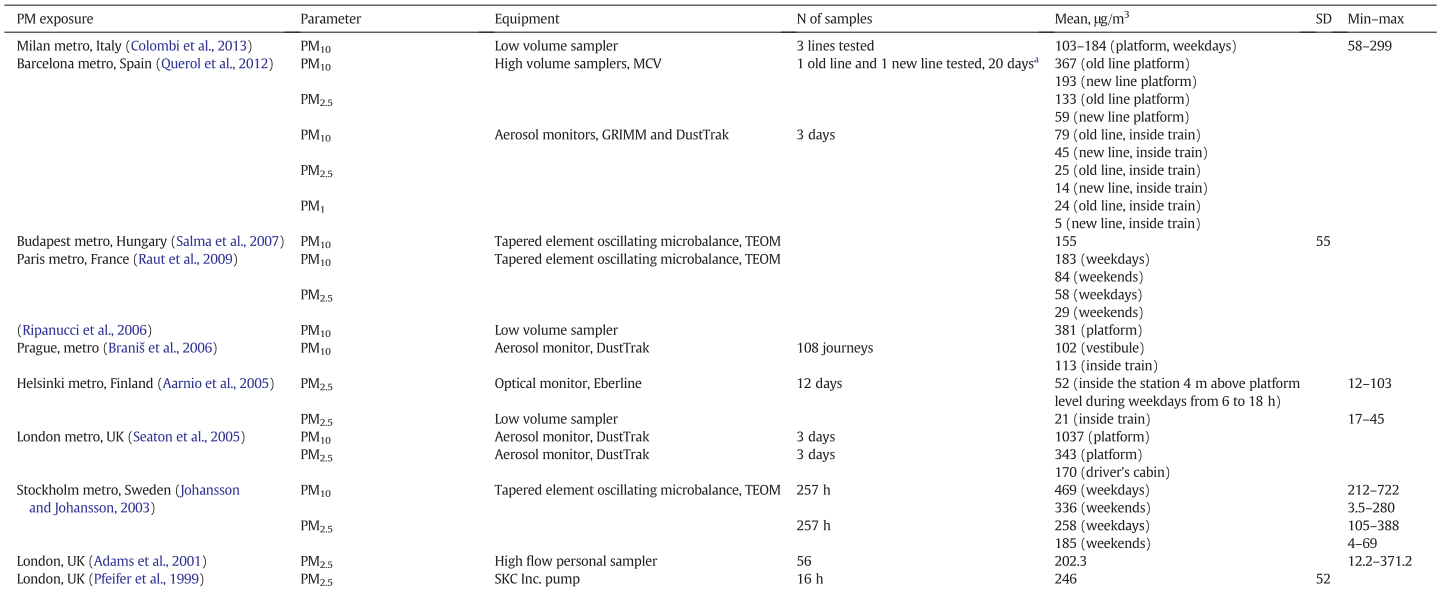
\includegraphics[scale=0.6]{pm_tube_summary}}
\caption{Summary of underground subway studies from \cite{Karanasiou2014}}
\label{fig:pm_tube_summary}
\end{figure}
\end{landscape}

Focusing specifically on London, the work of Adams in the late 1990's \slash early 2000's is oft cited and well known in this area of transport exposure due to it being the first comprehensive particulate matter multi--mode transport user exposure assessment study in the UK. They measured a large number of journeys (465) across many modes (bicycle, car, bus, tube) over different periods in July 1999 ('summer') and February 2000 ('winter') finding mean PM$_{2.5}$ values for the London Underground of 247.2 ug\slash /m\textsuperscript{3} in summer and 157.3 ug\slash m\textsuperscript{3} for the winter (or an overall mean of 202 ug\slash m\textsuperscript{3} as shown in the Figure \ref{fig:pm_tube_summary}). Shortly after this publication another paper was published by the same group which tried to apportion the PM to sources (\cite{Adams2001a}). They concluded that most of the PM came from metals from sources such as braking, tyre wear and the tracks. A high iron content was found. They noted that the PM in the underground should not be directly compared with PM above ground as it's composition is very different. In terms of the actual levels measured in the first paper however extrapolation of these measures across the entire underground network including within cabins and on the platforms is not proven. \cite{Seaton2005} found large variations between PM in cabins and on the platforms themselves. In their research (funded by the London Underground to look at at occupational health exposure to PM$_{2.5}$) platform concentrations were 270–-480 ug\slash m\textsuperscript{3} and cab concentrations were 130–-200 ug\slash m\textsuperscript{3}. Similarly high to the other studies of the London Underground. This paper also found a high iron content in the PM -- 67\%. Seaton summarises however that although the concentrations are high, they are unlikely to represent a health risk to workers. \cite{Loxham2013} disagrees. Their research was not included in the Karanasiou review (presumably due to it being published only shortly before the review). They looked at PM$_{10}$, PM$_{2.5}$ and PM$_{0.1}$ composition finding similar to the other research, that the particles are mostly from interaction between wheels, rails, and brakes with a high iron content. However they suggest that the potential health effects of exposure to the ultrafine fraction of underground PM warrants further investigation, as a consequence of its greater surface area/volume ratio and high metal content.

% LU summary bit.

To summarise, exposure and the related health effects of poor air quality in subway systems has not been extensively studied in most cities. Certainly not to the point where researchers can confidently say what levels of particulate matter the public are being exposed to at different times of the day, in different places of the underground, and what composition that has (and how toxic to the body it is or is not). What can be fairly confidently said however is that concentrations in most systems, and certainly in London, are higher than street-level, in-vehicle, cycling, buses or most other studied transport micro-environments. Although the composition is very different and may be more or less toxic. Due to the number of people that use this transport mode daily (1.171 billion journeys annually in London according to \cite{TransportforLondon2014a}) for extended periods of time, understanding and being able to quantify exposure during it is necessary to better estimate people's daily exposure across a range of micro-environments. Certainly they vary hugely from concentrations measured at a subjects place of residence, as is used in the static exposure studies considered earlier.

\vspace{1cm}

Studies of exposure while people are in-transit between locations using transport modes such as cars, trains, subway systems and bicycles shows a large range of concentration values. There are few exposure studies which account for these variations (alongside outdoor indoor infiltration) to provide exposure data on the daily lives of large numbers of subjects suitable for epidemiological analysis. Until more expansive exposure studies that follow large groups of people of varying time-activity patterns are completed, the ability to discern the range of commute-time’s specific contribution to total exposure is constrained (\cite{Knibbs2011}).
\newpage
%%%%%%%%%%%%%%%%%%%%%%%%%%%%%%%%%%%%%%%%
%%%%%%%%%%%%%% MODELLING %%%%%%%%%%%%%%%
%%%%%%%%%%%%%%%%%%%%%%%%%%%%%%%%%%%%%%%%

\subsection{Dynamic and Hybrid exposure models}
\label{sec:dynamic_hybrid_models}

Section \ref{sec:staticexposurehealth} (Static exposure studies) concluded that taking fixed-point or fixed-area measurements, often at one point in space or time, was insufficient to accurately quantify human exposure to air pollution. Exposures varies in space and time due to an individual’s activities, different sources having different effects, the time of day, and the location of the subject. For example the poor air an individual is exposed too will vary depending on how long they spend in public transport each day (and which mode of transport), how long they spend at home or at work, and the concentrations within those environments themselves (\cite{Ozkaynak2013}). Therefore models which look at these different environments, and their effects on health, are needed.

Section \ref{sec:personal_monitoring} (Personal monitoring) showed how personal monitoring devices could be used to better understand individual-level exposures, but was concluded by discussing how collecting enough accurate data using this method for large health studies is very difficult to do. The following Sections of \ref{sec:infiltration} (Infiltration) and \ref{sec:transport} (Transport) looked at models which enable researchers to quantify exposure to populations in those specific environments (and some discussed the health implications of those environments), but they were not 'joined-up' so as to enable estimates of total daily exposure alongside other micro-environments and times.

This section looks at a the small number of research studies which use models to attempt to be more holistic and include all micro-environments as well as temporal and spatial variation in their inputs. This is a new area of research which is not yet established, and the nomenclature is thus still under development, but a trend towards discussion of 'hybrid' or 'dynamic' models has emerged. 'Hybrid' being a description of a combining of multiple approaches of exposure, such as time-activity diaries combined with modelled air quality data and micro-environmental modelling of transport modes, and 'Dynamic' reflecting the improved temporal scale of data available, for both the populations movement and the variation in pollutant concentrations. Also discussed below are publications by \cite{Ozkaynak2013}, \cite{Meliker2011} and \cite{Baxter2013} who have attempted to advance this field by reviewing recent approaches and suggesting key areas which need to be improved, or by identifying what exactly these new types of model should do. 

%%%%%%%%%%%%
\cite{Kousa2002} was a very early attempt at this sort of model. They evaluated the temporal and spatial exposure of the population of the Helsinki Metropolitan Area in different micro-environments (home, workplace, traffic and other). For time-activity data (15 min resolution) they used 435 diaries from the EXPOLIS study, and they then linked this to modelled NO$_{2}$ data from a dispersion model which outputted grids of 500 m by 500 m for the greater Helsinki area, and 50 m by 50 m for the city centre. For indoor environments they took an I/O ratio of 0.76, including when the subjects were recorded as being in transport. The GIS technology and techniques used in this model would have been quite advanced at the time, and therefore modelling the exposure of 8000 people was impressive. Specifically, modelling the air quality with hourly variation and at 50 m resolution. However in-light of contemporary work this model is simplistic in a number of ways including: only describing four micro-environments (and using the same I\slash O ratio for all of them), that the time-activity diaries are only at 15 minute intervals, that the data only includes people of ages 25-55, and that the days modelled are only 'working days' i.e. Monday to Friday. It would also have been interesting to see what difference using this model made on exposure assessment i.e. a comparison with other methods - such as the research by \cite{Dhondt2012}. Based in Belgium they compared 'static' and 'dynamic' models for exposure for NO$_{2}$ and O$_{3}$, modelling their subject's behaviours and location based on 8800 activity diaries into 12 km location 'zones', then scaling this to give results relevant for 5 million people. For their air quality inputs hourly concentrations were modelled using a variety of nested models, giving higher resolution nearer to roads and in urban areas, and lower resolution outside of these areas. Time in transport in each zone was also included. Maps showing the exposure over 24 hours accumulated by each zone are shown in Figures \ref{fig:dhondt_static_exposure} and \ref{fig:dhondt_dynamic_exposure}.

\begin{figure}[H]
\centering
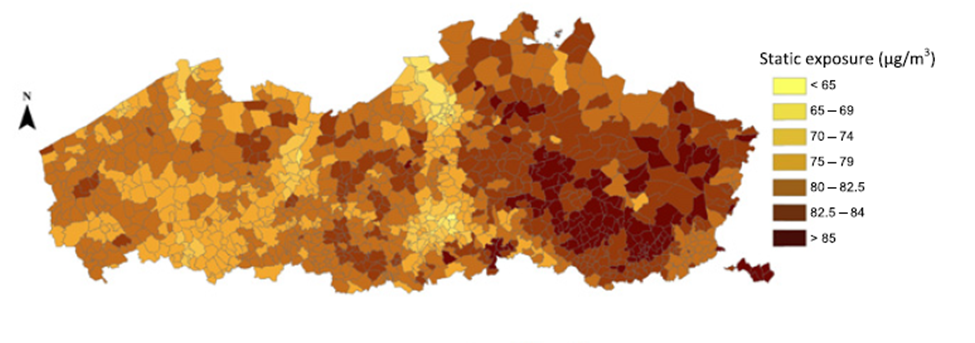
\includegraphics[scale=0.8]{dhondt_static_exposure}
\caption{NO$_{2}$ static exposure results from \cite{Dhondt2012}}
\label{fig:dhondt_static_exposure}
\end{figure}

\begin{figure}[H]
\centering
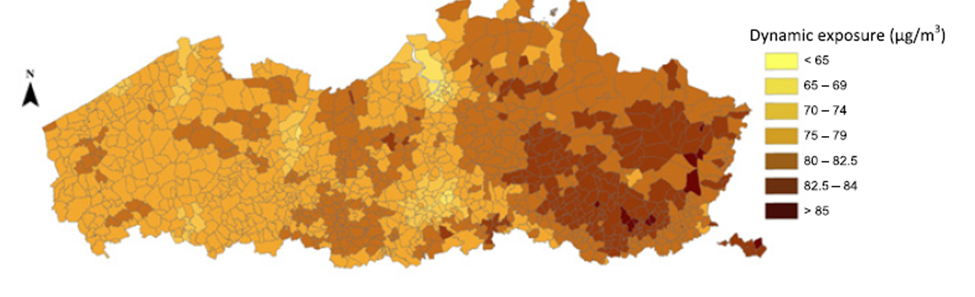
\includegraphics[scale=0.8]{dhondt_dynamic_exposure}
\caption{NO$_{2}$ dynamic exposure results from \cite{Dhondt2012}}
\label{fig:dhondt_dynamic_exposure}
\end{figure}

By using this approach to exposure modelling they found NO$_{2}$ was being underestimated by on average 1.2\%, and that O$_{3}$ was being overestimated by 0.8\%. These do not seem particularly large differences, however as an input to a large cohort of people in a long time-series analysis they could significantly change the health conclusions reached. These regional averages also mask much of the variation in individuals, where differences of upto 12\% can be found depending on age group, gender and place of residence. Having studied their methods however, the reliability of the results must be questioned. This research is certainly moving towards the type of dynamic exposure model described earlier, as their modelled air quality and time-activity data is of a high quality, however there is no micro-environmental modelling at all, which given the time that we know people spend indoors must be a large source of uncertainty in the results. As a final note on this publication, the method of grouping the exposure results into time-activity zones rather than by residence of the subject was interesting and informative, showing the areas where greatest miss-classification occurred in a simple, visual and effective manner.

%%%%%%%%%%%%
%% Study uses modelling of air quality and adjustments for micro-environments.
%% But difficult to upscale and relies on alot of context thus not good.

The following year \cite{DeNazelle2013} did a similar study for 7 days of 36 subjects in Barcelona, however in addition to using time-activity diaries as an input, the subjects also had software installed on a provided smartphone, which made use of the accelerometer and GPS hardware to record their location and infer their type of activity i.e. walking, sitting. After (substantial) processing of this data, the subjects location and activity was linked with an hourly resolved 5 km x 5 km dispersion model grid of NO$_{2}$, and personal exposure was then calculated -- including adjustments for six different micro-environments (indoor, bike, bus and tram, car and taxi, metro and train, motorcycle). This study was truly a hybrid study, in that data was collected using personal monitoring (smartphones) but then joined with modelled data and further processing of the data. De Nazelle then calculated the time that the subjects spent in different micro-environments, and compared this to the percentage of their daily exposure in the same micro-environment categories (Figure \ref{fig:time_no2_activity_spaces}).

\begin{figure}[H]
\centering
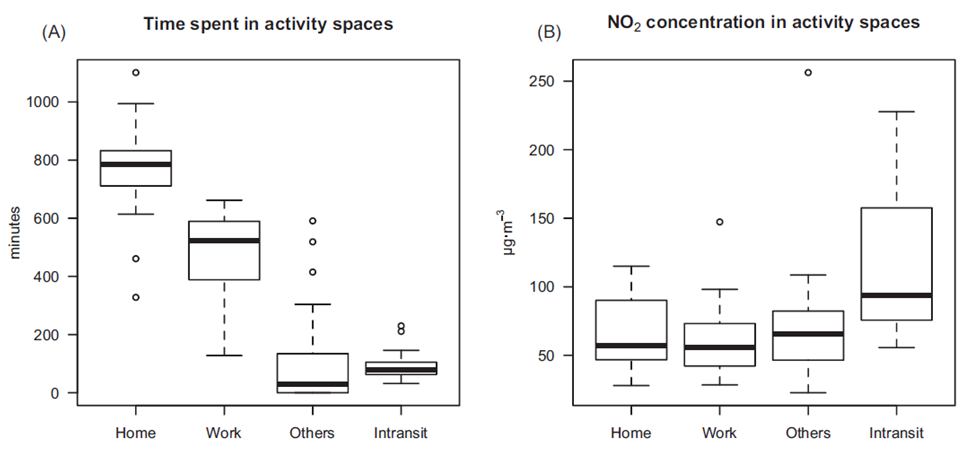
\includegraphics[scale=0.8]{time_no2_activity_spaces}
\caption{Time and NO$_{2}$ in activity spaces from \cite{DeNazelle2013}}
\label{fig:time_no2_activity_spaces}
\end{figure}

From the results we can see that in terms of minutes, the subjects spent most of their time at home and at work (left), supporting the use of static exposure models where these fixed locations are used, however when the actual exposure is considered the influence of the time spent in those locations diminishes (right) and 'Others' and 'Intransit' become important (supporting the conclusions of \cite{Dons2011} discussed in Section \ref{sec:transport}). The study concludes by discussing how these techniques that have been used could be developed and used for much larger populations (presumably as an input to health studies eventually) , however I would suggest that the amount of post-processing of the geographical data, the manual translation of activity diaries to compliment the smartphone data, and the extra battery packs that needed adding to the phones makes this seem less likely. To upscale this to many hundreds or thousands of subjects would need a tremendous amount of coordination and equipment which would need to be distributed, collected and monitored. The data processing would also seem to be difficult without large human resources, and linking to health outcomes would mean the study needed to be designed so that the participants are a statistical representation of the wider study area population, or the numbers surveyed so close to the actual study population that they give a good representation anyway. 

%%%%%%%%%%%%
In the same year \cite{Gerharz2013} used similar methods to examine the exposure of 10 people in Munster, Germany. They used activity diaries alongside GPS data again, defined micro-environments using this contextual information of 'home', 'work', 'other indoor', 'transportation', and 'outdoor', joined this to an hourly average PM$_{10}$ dispersion model for the air quality input, and then used I/O ratios for the micro-environments e.g. 1.34 for cars and 2.49 for public transport. The model is summarised in Figure \ref{fig:gerharz_exposure_diagram} below.

\begin{figure}[H]
\centering
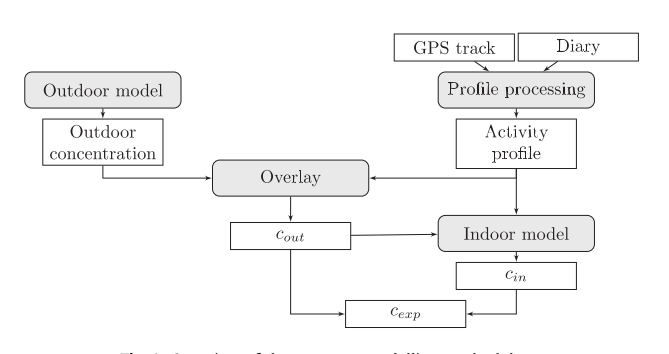
\includegraphics[scale=0.8]{gerharz_exposure_diagram}
\caption{The exposure process from \cite{Gerharz2013} }
\label{fig:gerharz_exposure_diagram}
\end{figure}

The major difference between this and the work of De Nazelle and Dons is that they also gave the subjects personal air quality monitoring data in the form of a Grimm Aerosol Spectrometer. The spectrometer provided information about particle numbers and mass in 32-size classes with a high temporal resolution of 6 seconds. Using this data they were able to evaluate the effectiveness of their modelled exposure by comparing it to real data. The Pearson’s correlation coefficient between the mean of modelled and measured data is shown in Figure \ref{fig:gerharz_results}.

\begin{figure}[H]
\centering
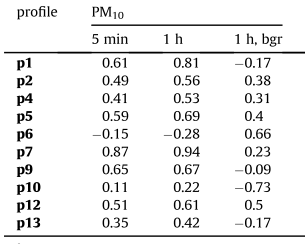
\includegraphics[scale=1]{gerharz_results}
\caption{Pearson’s correlation coefficient between the mean of modelled and measured data from \cite{Gerharz2013} }
\label{fig:gerharz_results}
\end{figure}

There is clearly some variation between the results, with P7 (person 7) being particularly strong, and P10 being particularly weak. Gerharz notes in their discussion that "Generally, the correlation between model average and measurements is high" which I would dispute with the mean of the correlations coming out as 0.44 i.e. Medium correlation. However they are correct in saying that it does at least "clearly outperforms the baseline approach of using urban background measurements as proxy for the personal exposure". Though in terms of using this modelled approach for larger groups of people, the post-processing of GPS data and activity-diaries, general data cleaning, and data linkage would seem to make this an unlikely approach.

%%%%%%%%%%%%
\cite{Ozkaynak2013}, \cite{Meliker2011} and \cite{Baxter2013} have written reviews / position statements on this type of research. Ozkaynak's diagram below (Figure \ref{fig:ozkaynak_exposure_diagram}) is useful for summarising how the complexity of exposure modelling has advanced, and with the complexity the inputs required.

\begin{figure}[H]
\centering
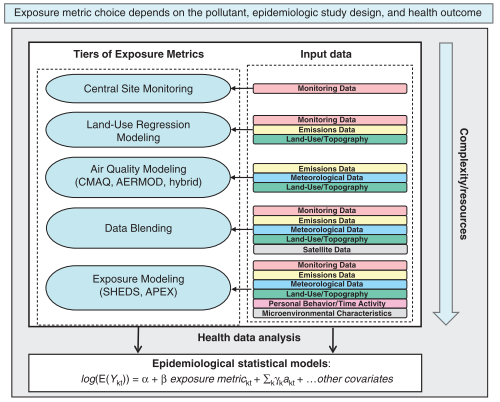
\includegraphics[scale=1]{ozkaynak_exposure_diagram}
\caption{The evolution of exposure assessment from \cite{Ozkaynak2013}}
\label{fig:ozkaynak_exposure_diagram}
\end{figure}

They concluded that these new approaches can help refine the significance of air pollution health outcomes, but that this will depend on study-specific characteristics, including epidemiological study design (e.g., time-series vs cohort), the form of of health outcome being considered (e.g., long-term or short-term), which pollutants, and the role of pollutant and building specific indoor infiltration and human activity patterns. \cite{Meliker2011} offers a slightly different but useful perspective, by identifying what they consider are the five most important domains to the development of improved spatio-temporal epidemiological models, namely:

\begin{enumerate}
  \item spatio-temporal epidemiologic theory
  \item selection of appropriate spatial scale of analysis
  \item choice of spatial/spatio-temporal method for pattern identification
  \item individual-level exposure assessment in epidemiologic studies
  \item assessment and consideration of locational and attribute uncertainty
\end{enumerate}

\cite{Baxter2013} summarises this emerging area of research well by explaining how, when compared with the use of central-site monitoring data (or other fixed-location methods) the enhanced spatial (and temporal) resolution of air quality or exposure models can impact on resultant health effect estimates, especially for pollutants derived from local sources such as traffic.  They recommend that future research develops pollutant-specific infiltration data, improves existing data on human time-activity patterns and exposure to local sources, in order to enhance human exposure modelling estimates. Also that these new approaches are compared with existing approaches to exposure estimation to better characterise estimates in chronic health studies.

\vspace{1cm}
%%%%%%%%%%%%
Figure \ref{fig:james_exposure_diagram} is proposed as a conceptual model of a hybrid/dynamic exposure model. It should have highly temporal and spatially resolved air quality inputs which consider both indoor and outdoor sources (including regional and local source for the latter), it should be able to model infiltration rates for different modes of transport and building types, it should reflect the multiple micro-environments that people spend their time in (and take account of the temporal resolution of these) and finally it should (for linkage through to epidemiological end-points) be able to consider different breathing rates to quantify exposure and dose for multiple pollutants.

\begin{figure}[H]
\centering
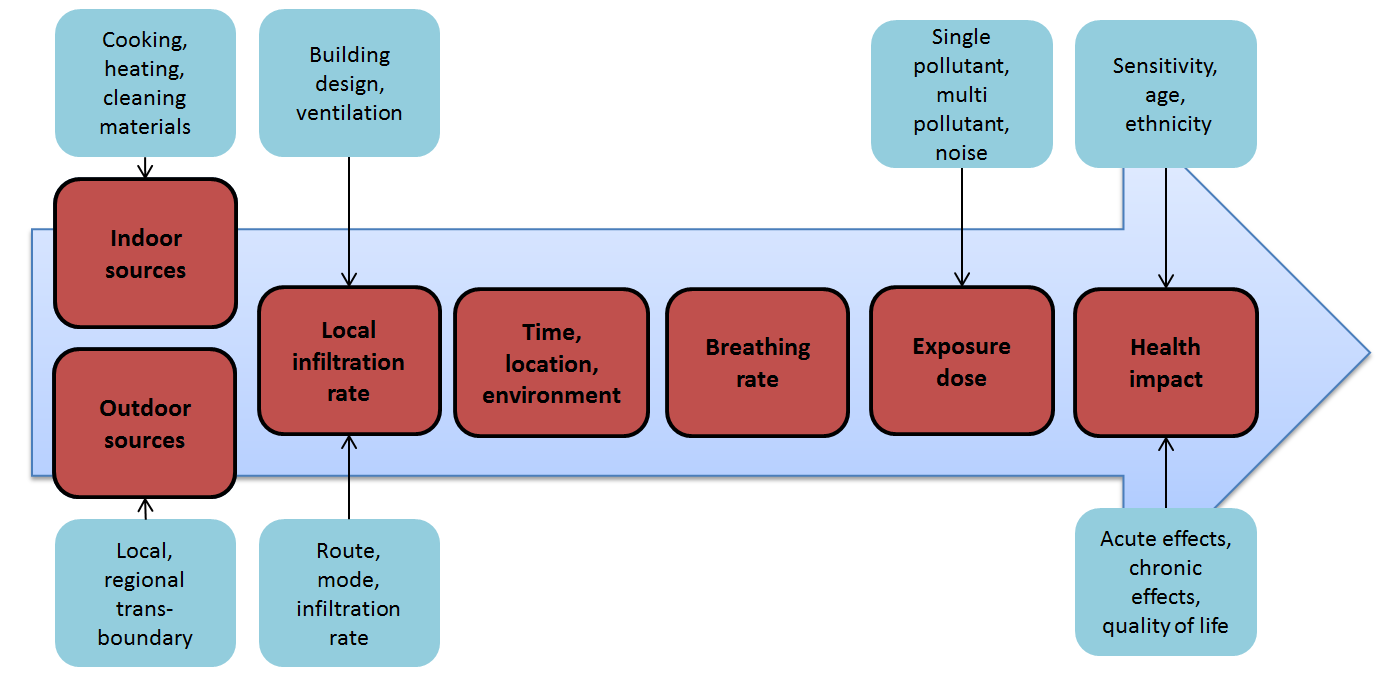
\includegraphics[scale=0.4]{james_exposure_diagram}
\caption{A conceptual dynamic exposure model}
\label{fig:james_exposure_diagram}
\end{figure}

%New studies to add when re-write this section near end of PhD
%\cite{Su2015}
%\cite{Schwartz2007}
%\cite{Di2017}